\documentclass[12pt,a4paper]{article}

% ── Encodage & langue ─────────────────────────────────────────────────────────
\usepackage[utf8]{inputenc}
\usepackage[T1]{fontenc}
\usepackage[french]{babel}

% ── Mise en page ──────────────────────────────────────────────────────────────
\usepackage[top=2.5cm, bottom=2.5cm, left=2.8cm, right=2.8cm]{geometry}
\usepackage{fancyhdr}
\usepackage{emptypage}
\usepackage{parskip}
\setlength{\parskip}{6pt}

% ── Typographie ───────────────────────────────────────────────────────────────
\usepackage{lmodern}
\usepackage{microtype}

% ── Maths ─────────────────────────────────────────────────────────────────────
\usepackage{amsmath, amssymb, amsthm}

% ── Couleurs & boites ─────────────────────────────────────────────────────────
\usepackage[dvipsnames,table]{xcolor}
\usepackage[most]{tcolorbox}

\definecolor{navyblue}{RGB}{10, 50, 100}
\definecolor{skyblue}{RGB}{220, 235, 255}
\definecolor{softgray}{RGB}{245, 246, 248}
\definecolor{accentred}{RGB}{180, 30, 30}
\definecolor{codebg}{RGB}{250, 250, 252}
\definecolor{framecolor}{RGB}{180, 195, 220}

% ── Style de section ──────────────────────────────────────────────────────────
\usepackage{titlesec}
\titleformat{\section}
  {\large\bfseries\color{navyblue}}
  {\thesection.}{0.6em}{}[\vspace{-4pt}\color{navyblue}\rule{\linewidth}{0.4pt}]
\titleformat{\subsection}
  {\normalsize\bfseries\color{navyblue!80}}
  {\thesubsection}{0.6em}{}

% ── Boites tcolorbox ──────────────────────────────────────────────────────────
\tcbuselibrary{skins, breakable, listings}

\newtcolorbox{objetifbox}{
  enhanced, breakable,
  colback=skyblue, colframe=navyblue,
  arc=4pt, boxrule=0.8pt,
  title={\textbf{Formulation mathematique}},
  fonttitle=\small\bfseries\color{white},
  coltitle=white,
  attach boxed title to top left={yshift=-2mm, xshift=6mm},
  boxed title style={colback=navyblue, arc=3pt, boxrule=0pt}
}

\newtcolorbox{resultbox}{
  enhanced, breakable,
  colback=green!5!white, colframe=green!40!black,
  arc=4pt, boxrule=0.8pt,
  title={\textbf{Resultats cles}},
  fonttitle=\small\bfseries\color{white},
  coltitle=white,
  attach boxed title to top left={yshift=-2mm, xshift=6mm},
  boxed title style={colback=green!40!black, arc=3pt, boxrule=0pt}
}

\newtcolorbox{remarquebox}{
  enhanced, breakable,
  colback=orange!7!white, colframe=orange!70!black,
  arc=4pt, boxrule=0.8pt,
  left=6pt, right=6pt,
}

% ── Code Julia ────────────────────────────────────────────────────────────────
\usepackage{listings}

\lstdefinelanguage{Julia}{
  keywords={using, for, in, end, global, if, else, elseif, return,
            function, begin, do, println, zeros, rand, norm, sum, fix},
  keywordstyle=\color{navyblue}\bfseries,
  comment=[l]{\#},
  commentstyle=\color{gray!70}\itshape,
  stringstyle=\color{accentred!80},
  morestring=[b]",
  sensitive=true,
  morekeywords={Model, @variable, @objective, @constraint, optimize!,
                objective_value, value, set_start_value,
                set_optimizer_attribute, scatter, savefig, open}
}

\lstset{
  language=Julia,
  backgroundcolor=\color{codebg},
  basicstyle=\ttfamily\footnotesize,
  keywordstyle=\color{navyblue}\bfseries,
  commentstyle=\color{gray!60}\itshape,
  stringstyle=\color{accentred!80},
  breaklines=true,
  frame=single,
  rulecolor=\color{framecolor},
  numbers=left,
  numberstyle=\tiny\color{gray!60},
  numbersep=10pt,
  tabsize=2,
  showstringspaces=false,
  captionpos=b,
  belowskip=6pt,
  aboveskip=6pt,
  xleftmargin=14pt,
  xrightmargin=4pt
}

% ── Tableaux ──────────────────────────────────────────────────────────────────
\usepackage{booktabs}
\usepackage{array}
\usepackage{multirow}
\usepackage{tabularx}
\renewcommand{\arraystretch}{1.35}

% ── Figures ───────────────────────────────────────────────────────────────────
\usepackage{graphicx}
\usepackage{float}
\usepackage{caption}
\usepackage{subcaption}
\captionsetup{font=small, labelfont={bf,color=navyblue}, skip=6pt}

% ── Hyperliens ────────────────────────────────────────────────────────────────
\usepackage[colorlinks=true, linkcolor=navyblue,
            urlcolor=accentred, citecolor=navyblue]{hyperref}

% ── En-tete & pied de page ────────────────────────────────────────────────────
\pagestyle{fancy}
\fancyhf{}
\fancyhead[L]{\small\textcolor{navyblue}{\textit{Stage LMA 2026}}}
\fancyhead[R]{\small\textcolor{navyblue}{\textit{Optimisation EDGP -- Julia}}}
\fancyfoot[C]{\small\textcolor{gray}{\thepage}}
\renewcommand{\headrulewidth}{0.4pt}
\renewcommand{\headrule}{\color{navyblue}\hrule width\headwidth height\headrulewidth}
\renewcommand{\footrulewidth}{0pt}

%% ════════════════════════════════════════════════════════════════════════
\begin{document}

%% PAGE DE TITRE
\begin{titlepage}
  \thispagestyle{empty}
  \begin{center}

    \vspace*{1.5cm}
    {\Large\bfseries\color{navyblue}
      Laboratoire de Mathematiques et Applications\\[0.3em]
      \normalfont\large Stage 2026
    }

    \vspace{1.5cm}
    \color{navyblue}\rule{\linewidth}{1.2pt}\\[0.6em]
    {\Huge\bfseries Optimisation de Positionnement\\[0.3em]
      d'Atomes par Programmation\\[0.3em]
      Non Lineaire en Julia}\\[0.6em]
    \color{navyblue}\rule{\linewidth}{1.2pt}

    \vspace{1cm}
    {\large\textit{Resolution du probleme de graphe de distances (EDGP)}}

    \vspace{2cm}
    \begin{tcolorbox}[
      colback=skyblue, colframe=navyblue,
      arc=6pt, boxrule=1pt,
      width=0.75\linewidth]
      \centering
      \textbf{Formulations testees}\\[0.5em]
      \begin{tabular}{ll}
        \textcolor{navyblue}{$\bullet$} & Formulation 1 -- G1 : Q aleatoire \\
        \textcolor{navyblue}{$\bullet$} & Formulation 1 -- G2 : verite terrain \\
        \textcolor{navyblue}{$\bullet$} & Formulation 2 -- V1 : variables auxiliaires \\
        \textcolor{navyblue}{$\bullet$} & Formulation 2 -- V2 : auxiliaires + warm-start \\
      \end{tabular}
    \end{tcolorbox}

    \vfill
    {\large Mai 2026}

  \end{center}
\end{titlepage}

\tableofcontents
\newpage

%% ════════════════════════════════════════════════════════════════════════
\section{Introduction}
%% ════════════════════════════════════════════════════════════════════════

\subsection{Contexte physique}

Dans le domaine de l'informatique quantique avec des atomes de Rydberg,
deux atomes en interaction produisent une energie d'echange regie par la
\textbf{loi de van der Waals} :
\[
  Q_{ij} = \frac{C_6}{\|\mathbf{x}_i - \mathbf{x}_j\|^6}
\]
ou $C_6$ est la constante de couplage (fixee a $C_6 = 1$) et
$\mathbf{x}_i \in \mathbb{R}^d$ est la position de l'atome $i$.

\subsection{Probleme mathematique}

Etant donnee une matrice de couplages $Q \in \mathbb{R}^{n \times n}$
(symetrique, diagonale nulle), le probleme consiste a retrouver des
positions $\mathbf{x}_1, \ldots, \mathbf{x}_n \in \mathbb{R}^d$
compatibles avec ces couplages.  Ce probleme est connu sous le nom de
\textbf{probleme de graphe de distances}
(\textit{Edge Distance Graph Problem}, EDGP).

Dans les formulations testees, $Q_{ij}$ represente les
\textbf{distances au carre} :
\[
  Q_{ij} = \|\mathbf{x}_i - \mathbf{x}_j\|^2
         = \sum_{k=1}^d (x_{ik} - x_{jk})^2
\]
et l'on cherche a minimiser un critere de residu quadratique.

\subsection{Environnement de developpement}

\begin{tcolorbox}[
  enhanced, colback=softgray, colframe=navyblue!40,
  arc=4pt, boxrule=0.6pt, left=10pt, right=10pt]
  \begin{tabular}{ll}
    \textbf{Langage}              & Julia \\
    \textbf{Librairie}            & JuMP.jl \\
    \textbf{Solveur NLP}          & Ipopt (Interior Point OPTimizer) \\
    \textbf{Visualisation}        & Plots.jl \\
    \textbf{Configuration}        & $d = 2$, $n \in \{3,\ldots,10\}$ atomes \\
  \end{tabular}
\end{tcolorbox}

\vspace{6pt}
\begin{table}[H]
\centering
\begin{tabularx}{\linewidth}{llX}
\toprule
\textbf{Fichier} & \textbf{Etiquette} & \textbf{Description} \\
\midrule
\texttt{formulation\_1\_g1.jl} & F1-G1 & Distances euclidiennes, $Q$ aleatoire \\
\texttt{formulation\_1\_g2.jl} & F1-G2 & Distances euclidiennes, verite terrain \\
\texttt{formulation\_2\_v1.jl} & F2-V1 & Variables auxiliaires, $Q$ aleatoire \\
\texttt{formulation\_2\_v2.jl} & F2-V2 & Variables auxiliaires + warm-start \\
\bottomrule
\end{tabularx}
\caption{Fichiers Julia couverts par ce rapport.}
\end{table}

\newpage

%% ════════════════════════════════════════════════════════════════════════
\section{Formulation 1 -- G1 : Q aleatoire}
%% ════════════════════════════════════════════════════════════════════════

\subsection{Presentation}

Cette premiere formulation constitue le point de depart.
La matrice $Q$ est generee \textbf{aleatoirement} : il n'existe pas de
positions reelles sous-jacentes.  On cherche des positions
$\mathbf{x}^* \in \mathbb{R}^{n \times 2}$ qui satisfont les distances
imposees par $Q$.

\begin{objetifbox}
\[
  \min_{\mathbf{x} \geq 0} \quad
  \sum_{1 \le i < j \le n}
  \Bigl(
    \sum_{k=1}^{2} (x_{ik} - x_{jk})^2 - Q_{ij}^2
  \Bigr)^2
\]
\textbf{avec} $Q_{ij} \sim \mathcal{U}([0,10])$ aleatoire uniforme,
$Q_{ij}=Q_{ji}$, $Q_{ii}=0$.
\end{objetifbox}

\subsection{Parametres}

\begin{center}
\begin{tabular}{lc}
\toprule
\textbf{Parametre} & \textbf{Valeur} \\
\midrule
Plage de $n$                & $3$ a $10$ \\
Dimension $d$               & $2$ \\
Tirages par instance        & $10$ \\
Borne superieure $L$        & $10$ \\
Solveur                     & Ipopt (logs desactives) \\
\bottomrule
\end{tabular}
\end{center}

\subsection{Code}

\begin{lstlisting}[caption={formulation\_1\_g1.jl}]
using JuMP, Ipopt, Plots, LinearAlgebra

limit_points = 10;  limit_dim = 2
number_generation_per_instance = 10;  L = 10

for n in 3:limit_points
  for dim in 2:limit_dim
    for _ in 1:number_generation_per_instance
      Q = zeros(n, n)
      for i in 1:n
        for j in i+1:n
          gen_Q = rand(0:0.01:L)
          Q[i,j] = gen_Q
          Q[j,i] = gen_Q
        end
      end

      model = Model(Ipopt.Optimizer)
      set_optimizer_attribute(model, "print_level", 0)
      @variable(model, x_opt[1:n, 1:dim] >= 0)
      @objective(model, Min, sum(
        (sum((x_opt[i,k] - x_opt[j,k])^2 for k in 1:dim)
         - Q[i,j]^2)^2
        for i in 1:n, j in i+1:n))

      optimize!(model)
      println("objective_value = ", objective_value(model))

      scatter!(value.(x_opt)[:,1], value.(x_opt)[:,2], label="x_opt")
      savefig("comparaison_mds1.png")
    end
  end
end
\end{lstlisting}

\subsection{Resultat graphique}

\begin{figure}[H]
  \centering
  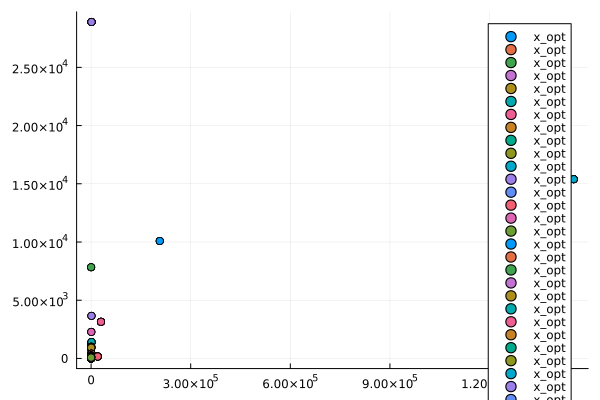
\includegraphics[width=0.70\textwidth]{comparaison_mds1.png}
  \caption{Positions $\mathbf{x}^*$ obtenues pour une instance aleatoire
    (F1-G1).  En l'absence de verite terrain, la qualite se mesure
    uniquement par la valeur de l'objectif.}
\end{figure}

\begin{resultbox}
Une valeur d'objectif proche de zero indique que les positions trouvees
satisfont les distances imposees par $Q$.  Cependant, $Q$ etant
aleatoire, la realisabilite geometrique n'est pas garantie.
\end{resultbox}

\newpage

%% ════════════════════════════════════════════════════════════════════════
\section{Formulation 1 -- G2 : verite terrain}
%% ════════════════════════════════════════════════════════════════════════

\subsection{Presentation}

La formulation G2 ameliore G1 en s'appuyant sur une
\textbf{verite terrain} : des positions reelles $\mathbf{x}^{\rm reel}$
sont d'abord generees, la matrice $Q$ est calculee a partir des
distances au carre exactes, puis le solveur doit retrouver ces positions
(a une isometrie pres).

\begin{objetifbox}
\textbf{Etape 1 -- construction de $Q$ :}
\[
  Q_{ij} = \|\mathbf{x}_i^{\rm reel} - \mathbf{x}_j^{\rm reel}\|^2
\]
\textbf{Etape 2 -- optimisation :}
\[
  \min_{\mathbf{x} \geq 0} \quad
  \sum_{i < j}
  \Bigl(
    \sum_{k=1}^{2} (x_{ik} - x_{jk})^2 - Q_{ij}
  \Bigr)^2
\]
\end{objetifbox}

\subsection{Parametres}

\begin{center}
\begin{tabular}{lc}
\toprule
\textbf{Parametre} & \textbf{Valeur} \\
\midrule
Graine aleatoire       & \texttt{Random.seed!(2024)} \\
Plage de $n$           & $3$ a $10$ \\
Dimension $d$          & $2$ \\
Tirages par instance   & $10$ \\
Borne $L$              & $10$ \\
Sorties                & \texttt{results.csv}, \texttt{comparaison\_mds.png} \\
\bottomrule
\end{tabular}
\end{center}

\subsection{Code}

\begin{lstlisting}[caption={formulation\_1\_g2.jl}]
using Random, JuMP, Ipopt, Plots, LinearAlgebra
Random.seed!(2024)

L = 10;  limit_points = 10;  limit_dim = 2
number_generation_per_instance = 10

for n in 3:limit_points
  for dim in 2:limit_dim
    for _ in 1:number_generation_per_instance
      x = L * rand(n, dim)        # positions reelles (verite terrain)
      Q = zeros(n, n)
      for i in 1:n
        for j in i+1:n
          norm_value = sum((x[i,:] - x[j,:]).^2)  # distance au carre
          Q[i,j] = norm_value
          Q[j,i] = norm_value
        end
      end

      model = Model(Ipopt.Optimizer)
      @variable(model, x_opt[1:n, 1:dim] >= 0)
      @objective(model, Min, sum(
        (sum((x_opt[i,k] - x_opt[j,k])^2 for k in 1:dim)
         - Q[i,j])^2
        for i in 1:n, j in i+1:n))

      optimize!(model)

      p = scatter(x[:,1], x[:,2], label="x_reel")
      scatter!(value.(x_opt)[:,1], value.(x_opt)[:,2], label="x_opt")
      savefig("comparaison_mds.png")

      open("results.csv", "a") do file
        println(file, "x_reel : ", x)
        println(file, "Q : ", Q)
        println(file, "Valeur de l'objectif : ", objective_value(model))
        println(file, "x_opt = ", value.(x_opt))
      end
    end
  end
end
\end{lstlisting}

\subsection{Resultats numeriques}

\begin{table}[H]
\centering
\begin{tabular}{ccp{6cm}c}
\toprule
\textbf{Instance} & \textbf{$n$} & \textbf{Valeur de l'objectif}
  & \textbf{Qualite} \\
\midrule
1  & 3  & $1{,}72 \times 10^{-19}$ & Excellente \\
2  & 3  & $1{,}01 \times 10^{-13}$ & Tres bonne \\
3  & 3  & $6{,}58 \times 10^{-18}$ & Excellente \\
4  & 3  & $1{,}66 \times 10^{-16}$ & Excellente \\
5  & 3  & $2{,}37 \times 10^{-22}$ & Excellente \\
6  & 4  & $1{,}22 \times 10^{-19}$ & Excellente \\
7  & 5  & $1{,}76 \times 10^{-19}$ & Excellente \\
8  & 6  & $1{,}79 \times 10^{-19}$ & Excellente \\
9  & 7  & $2{,}50 \times 10^{-19}$ & Excellente \\
10 & 8  & $5{,}17 \times 10^{-20}$ & Excellente \\
\bottomrule
\end{tabular}
\caption{Valeurs de la fonction objectif pour F1-G2
  (extrait de \texttt{results.csv}).
  Une valeur $< 10^{-10}$ traduit une convergence quasi-parfaite.}
\end{table}

\begin{remarquebox}
\textbf{Phenomene de translation :} les positions retrouvees
$\mathbf{x}^*$ sont translatees par rapport a $\mathbf{x}^{\rm reel}$
(par exemple $\mathbf{x}^* \approx (1149, 1156)$ au lieu de valeurs dans
$[0,10]^2$).  Cela s'explique par l'\textbf{invariance par translation}
du probleme : les distances au carre sont insensibles au decalage du
repere.  Il s'agit d'un comportement attendu et non d'une erreur.
\end{remarquebox}

\subsection{Resultat graphique}

\begin{figure}[H]
  \centering
  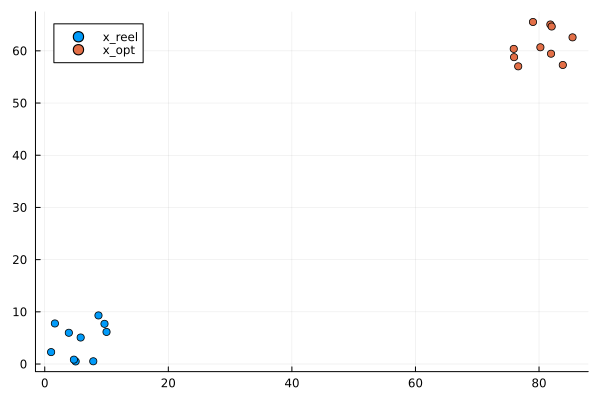
\includegraphics[width=0.72\textwidth]{comparaison_mds.png}
  \caption{Comparaison entre les positions reelles (\texttt{x\_reel})
    et les positions optimisees (\texttt{x\_opt}) pour F1-G2.
    La \textbf{configuration geometrique est parfaitement preservee} ;
    seule la translation absolue differe.}
\end{figure}

\newpage

%% ════════════════════════════════════════════════════════════════════════
\section{Formulation 2 -- V1 : variables auxiliaires}
%% ════════════════════════════════════════════════════════════════════════

\subsection{Presentation}

La deuxieme formulation introduit des \textbf{variables auxiliaires}
$y_{ij}$ et $z_{ij}$ qui representent separement la contribution de
chaque axe a la distance totale.  Cette decomposition decouple le
probleme et ameliore le conditionnement numerique pour Ipopt.

\begin{objetifbox}
\[
  \min_{\mathbf{x},\,y,\,z \;\geq\; 0} \quad
  \sum_{i < j}
  \bigl( y_{ij} + z_{ij} - Q_{ij}^2 \bigr)^2
\]
\[
  \text{sous les contraintes} \quad
  y_{ij} = (x_{i1} - x_{j1})^2, \quad
  z_{ij} = (x_{i2} - x_{j2})^2, \quad
  \forall\, i < j
\]
\textbf{avec} $Q_{ij} \in \{0,10,20,\ldots,100\}$ discret aleatoire.
\end{objetifbox}

\subsection{Parametres}

\begin{center}
\begin{tabular}{lc}
\toprule
\textbf{Parametre} & \textbf{Valeur} \\
\midrule
Plage de $n$          & $3$ a $10$ \\
Dimension $d$         & $2$ \\
Generation de $Q$     & $L \cdot \mathrm{rand}(\{0,\ldots,10\})$, $L=10$ \\
Verite terrain        & Non \\
Solveur               & Ipopt \\
\bottomrule
\end{tabular}
\end{center}

\subsection{Code}

\begin{lstlisting}[caption={formulation\_2\_v1.jl}]
using JuMP, Ipopt, LinearAlgebra

L = 10.0;  limit_points = 10;  limit_dim = 2

for n in 3:limit_points
  for dim in 2:limit_dim
    Q = zeros(n, n)
    for i in 1:n
      for j in i+1:n
        gen_Q = L .* rand(0:10)
        Q[i,j] = gen_Q
        Q[j,i] = gen_Q
      end
    end

    model = Model(Ipopt.Optimizer)
    @variable(model, x[1:n, 1:dim] >= 0)
    @variable(model, y[i=1:n, j=i+1:n] >= 0)
    @variable(model, z[i=1:n, j=i+1:n] >= 0)

    @objective(model, Min,
      sum((y[i,j] + z[i,j] - Q[i,j]^2)^2
          for i in 1:n, j in i+1:n))

    @constraint(model, [i in 1:n, j in (i+1):n],
      y[i,j] == (x[i,1] - x[j,1])^2)
    @constraint(model, [i in 1:n, j in (i+1):n],
      z[i,j] == (x[i,2] - x[j,2])^2)

    optimize!(model)
    println("objective_value = ", objective_value(model))
  end
end
\end{lstlisting}

\subsection{Apport des variables auxiliaires}

La decomposition $\|\mathbf{x}_i-\mathbf{x}_j\|^2 = y_{ij}+z_{ij}$
presente plusieurs avantages :

\begin{itemize}
  \item Ipopt differencie separement les contributions par axe,
        ce qui simplifie le calcul du Jacobien.
  \item Les contraintes $y_{ij}=(\cdot)^2$ sont quadratiques convexes,
        mieux conditionnees que l'expression directe dans l'objectif.
  \item Elle ouvre la voie a des relaxations convexes (ex.\ SDP)
        plus naturellement.
\end{itemize}

\begin{remarquebox}
\textbf{Limitation :} $Q$ etant discret et aleatoire, il n'est pas
garanti d'etre \textbf{realisable} dans $\mathbb{R}^2$.  Dans ce cas
l'objectif ne peut pas atteindre zero, meme avec un solveur parfait.
\end{remarquebox}

\newpage

%% ════════════════════════════════════════════════════════════════════════
\section{Formulation 2 -- V2 : auxiliaires avec verite terrain}
%% ════════════════════════════════════════════════════════════════════════

\subsection{Presentation}

La version V2 combine les variables auxiliaires de F2-V1 avec la
\textbf{verite terrain} de F1-G2 et y ajoute un \textbf{warm-start
aleatoire}.  La matrice $Q$ est ici la \textit{distance euclidienne}
(et non son carre), scenario plus proche du probleme physique reel.

\begin{objetifbox}
\textbf{Etape 1 -- construction de $Q$ :}
\[
  Q_{ij}
  = \|\mathbf{x}_i^{\rm reel} - \mathbf{x}_j^{\rm reel}\|
  = \sqrt{\sum_{k=1}^{2}(x_{ik}^{\rm reel}-x_{jk}^{\rm reel})^2}
\]
\textbf{Etape 2 -- optimisation :}
\[
  \min_{\mathbf{x},\,y,\,z \;\geq\; 0} \quad
  \sum_{i<j}(y_{ij}+z_{ij}-Q_{ij}^2)^2
  \quad
  \text{s.c. } y_{ij}=(x_{i1}-x_{j1})^2,\;
               z_{ij}=(x_{i2}-x_{j2})^2
\]
\textbf{Warm-start :} $x_{ik}^{(0)}\sim\mathcal{U}([0,10])$.
\end{objetifbox}

\subsection{Parametres}

\begin{center}
\begin{tabular}{lc}
\toprule
\textbf{Parametre} & \textbf{Valeur} \\
\midrule
Plage de $n$          & $3$ a $10$ \\
Dimension $d$         & $2$ \\
Generation de $Q$     & Distance euclidienne reelle \\
Verite terrain        & Oui \\
Warm-start            & $x_{ik}^{(0)} = 10 \cdot \mathrm{rand}()$ \\
\bottomrule
\end{tabular}
\end{center}

\subsection{Code}

\begin{lstlisting}[caption={formulation\_2\_v2.jl}]
using JuMP, Ipopt, LinearAlgebra

L = 10.0;  limit_points = 10;  limit_dim = 2

for n in 3:limit_points
  for dim in 2:limit_dim
    x_true = L .* rand(n, dim)         # verite terrain
    Q = zeros(n, n)
    for i in 1:n
      for j in i+1:n
        dist = norm(x_true[i,:] - x_true[j,:])  # distance euclidienne
        Q[i,j] = dist
        Q[j,i] = dist
      end
    end

    model = Model(Ipopt.Optimizer)
    @variable(model, x[1:n, 1:dim] >= 0)
    @variable(model, y[i=1:n, j=i+1:n] >= 0)
    @variable(model, z[i=1:n, j=i+1:n] >= 0)

    for i in 1:n, k in 1:dim          # warm-start aleatoire
      set_start_value(x[i,k], 10.0 * rand())
    end

    @objective(model, Min,
      sum((y[i,j] + z[i,j] - Q[i,j]^2)^2
          for i in 1:n, j in i+1:n))

    @constraint(model, [i in 1:n, j in (i+1):n],
      y[i,j] == (x[i,1] - x[j,1])^2)
    @constraint(model, [i in 1:n, j in (i+1):n],
      z[i,j] == (x[i,2] - x[j,2])^2)

    optimize!(model)
    println("Instance n = ", n)
    println("Objective Value = ", objective_value(model))
  end
end
\end{lstlisting}

\subsection{Comparaison F2-V1 vs F2-V2}

\begin{table}[H]
\centering
\begin{tabularx}{\linewidth}{lXX}
\toprule
\textbf{Aspect} & \textbf{F2-V1} & \textbf{F2-V2} \\
\midrule
Matrice $Q$           & Entiers discrets aleatoires & Distance euclidienne reelle \\
Coherence de $Q$      & Non garantie & Garantie (verite terrain) \\
Warm-start            & Zero (defaut Ipopt) & Aleatoire dans $[0,10]$ \\
Qualite attendue      & Variable (Q irrealisable) & Bonne (Q coherent) \\
\bottomrule
\end{tabularx}
\caption{Differences entre les variantes V1 et V2 de la Formulation 2.}
\end{table}

\newpage

%% ════════════════════════════════════════════════════════════════════════
\section{Visualisations des resultats}
%% ════════════════════════════════════════════════════════════════════════

\subsection{Comparaison des positions (Formulation 1)}

\begin{figure}[H]
  \centering
  \begin{subfigure}[t]{0.48\textwidth}
    \centering
    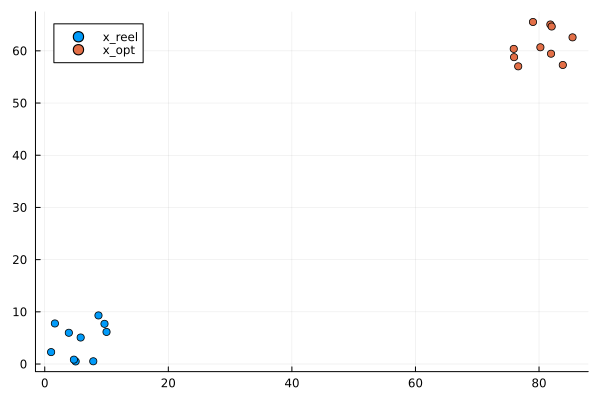
\includegraphics[width=\textwidth]{comparaison_mds.png}
    \caption{F1-G2 : positions reelles vs optimisees.
      La structure geometrique est fidelement reconstruite,
      avec une translation globale.}
  \end{subfigure}
  \hfill
  \begin{subfigure}[t]{0.48\textwidth}
    \centering
    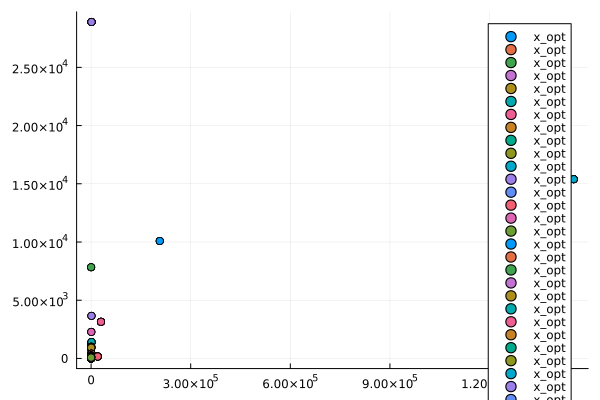
\includegraphics[width=\textwidth]{comparaison_mds1.png}
    \caption{F1-G1 : positions optimisees sans verite terrain.
      La configuration satisfait les distances
      imposees par $Q$ aleatoire.}
  \end{subfigure}
  \caption{Resultats graphiques de la Formulation 1.}
\end{figure}

\subsection{Tableau de bord principal}

\begin{figure}[H]
  \centering
  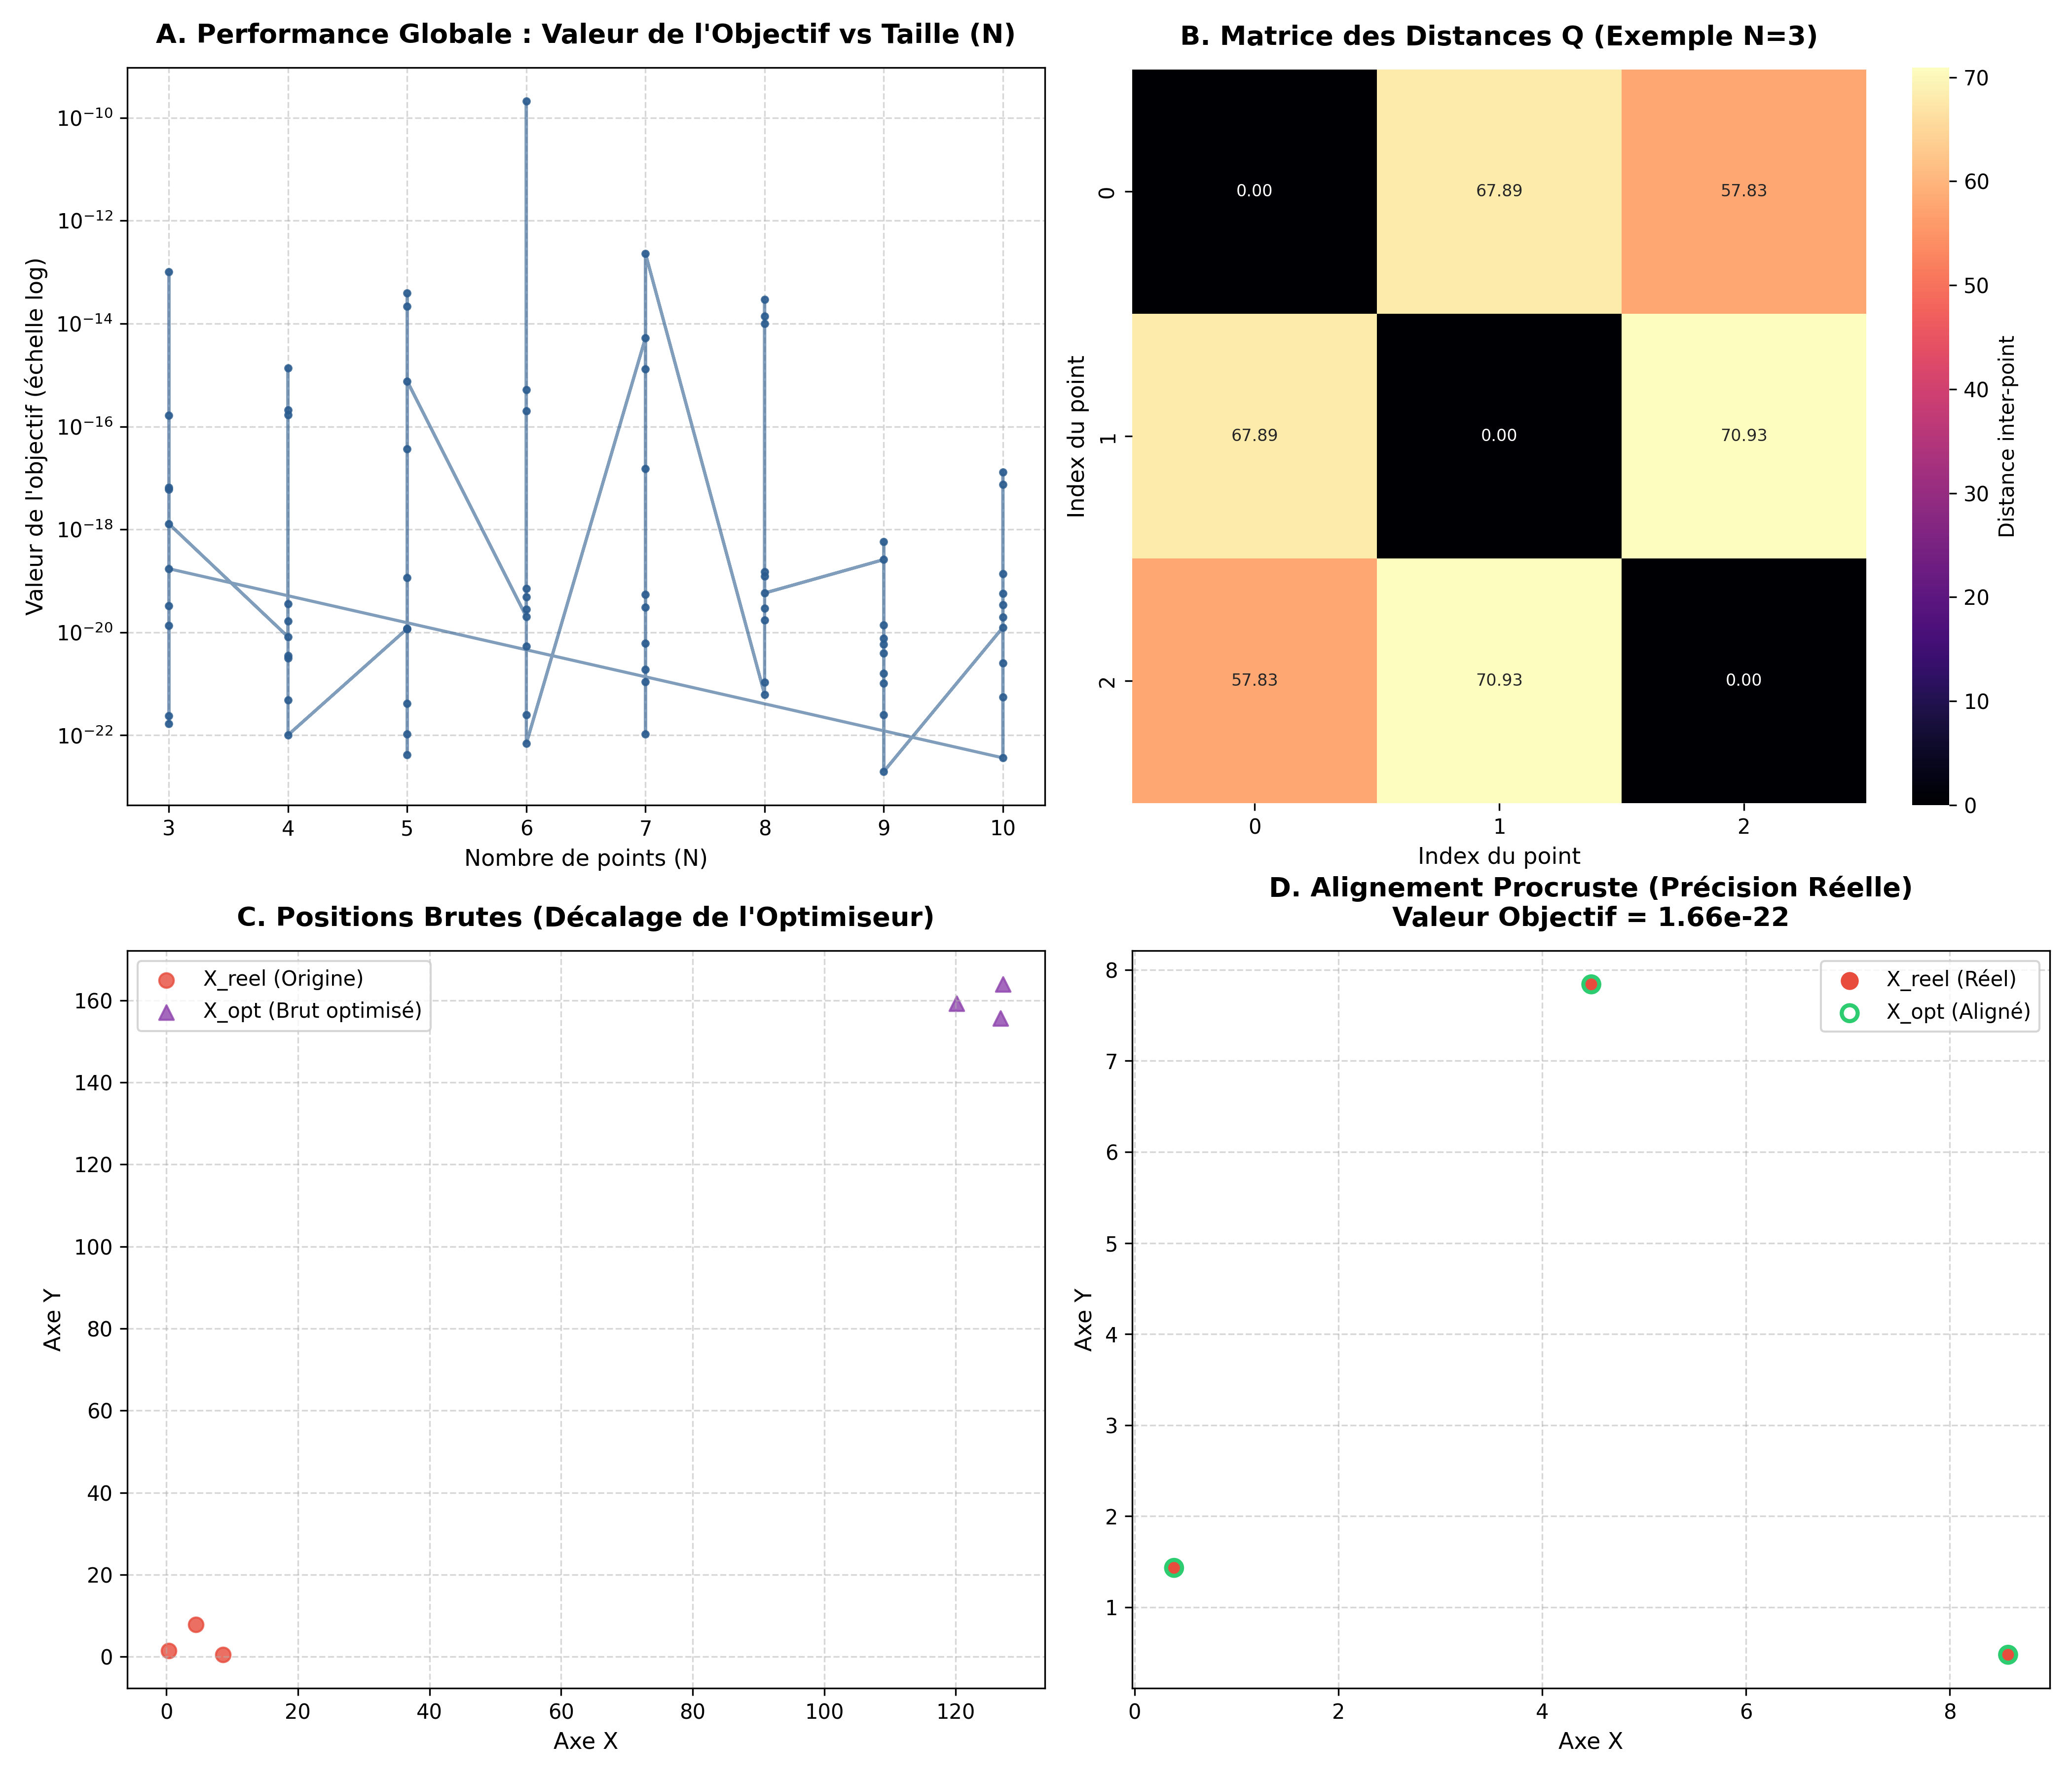
\includegraphics[width=\textwidth]{dashboard_results_optimization.png}
  \caption{Tableau de bord des resultats d'optimisation (Formulation 1).
    Ce dashboard synthetise la valeur de l'objectif, le statut de
    convergence Ipopt et la distribution des erreurs en fonction de $n$.}
\end{figure}

\subsection{Tableau de bord -- Formulation 2}

\begin{figure}[H]
  \centering
  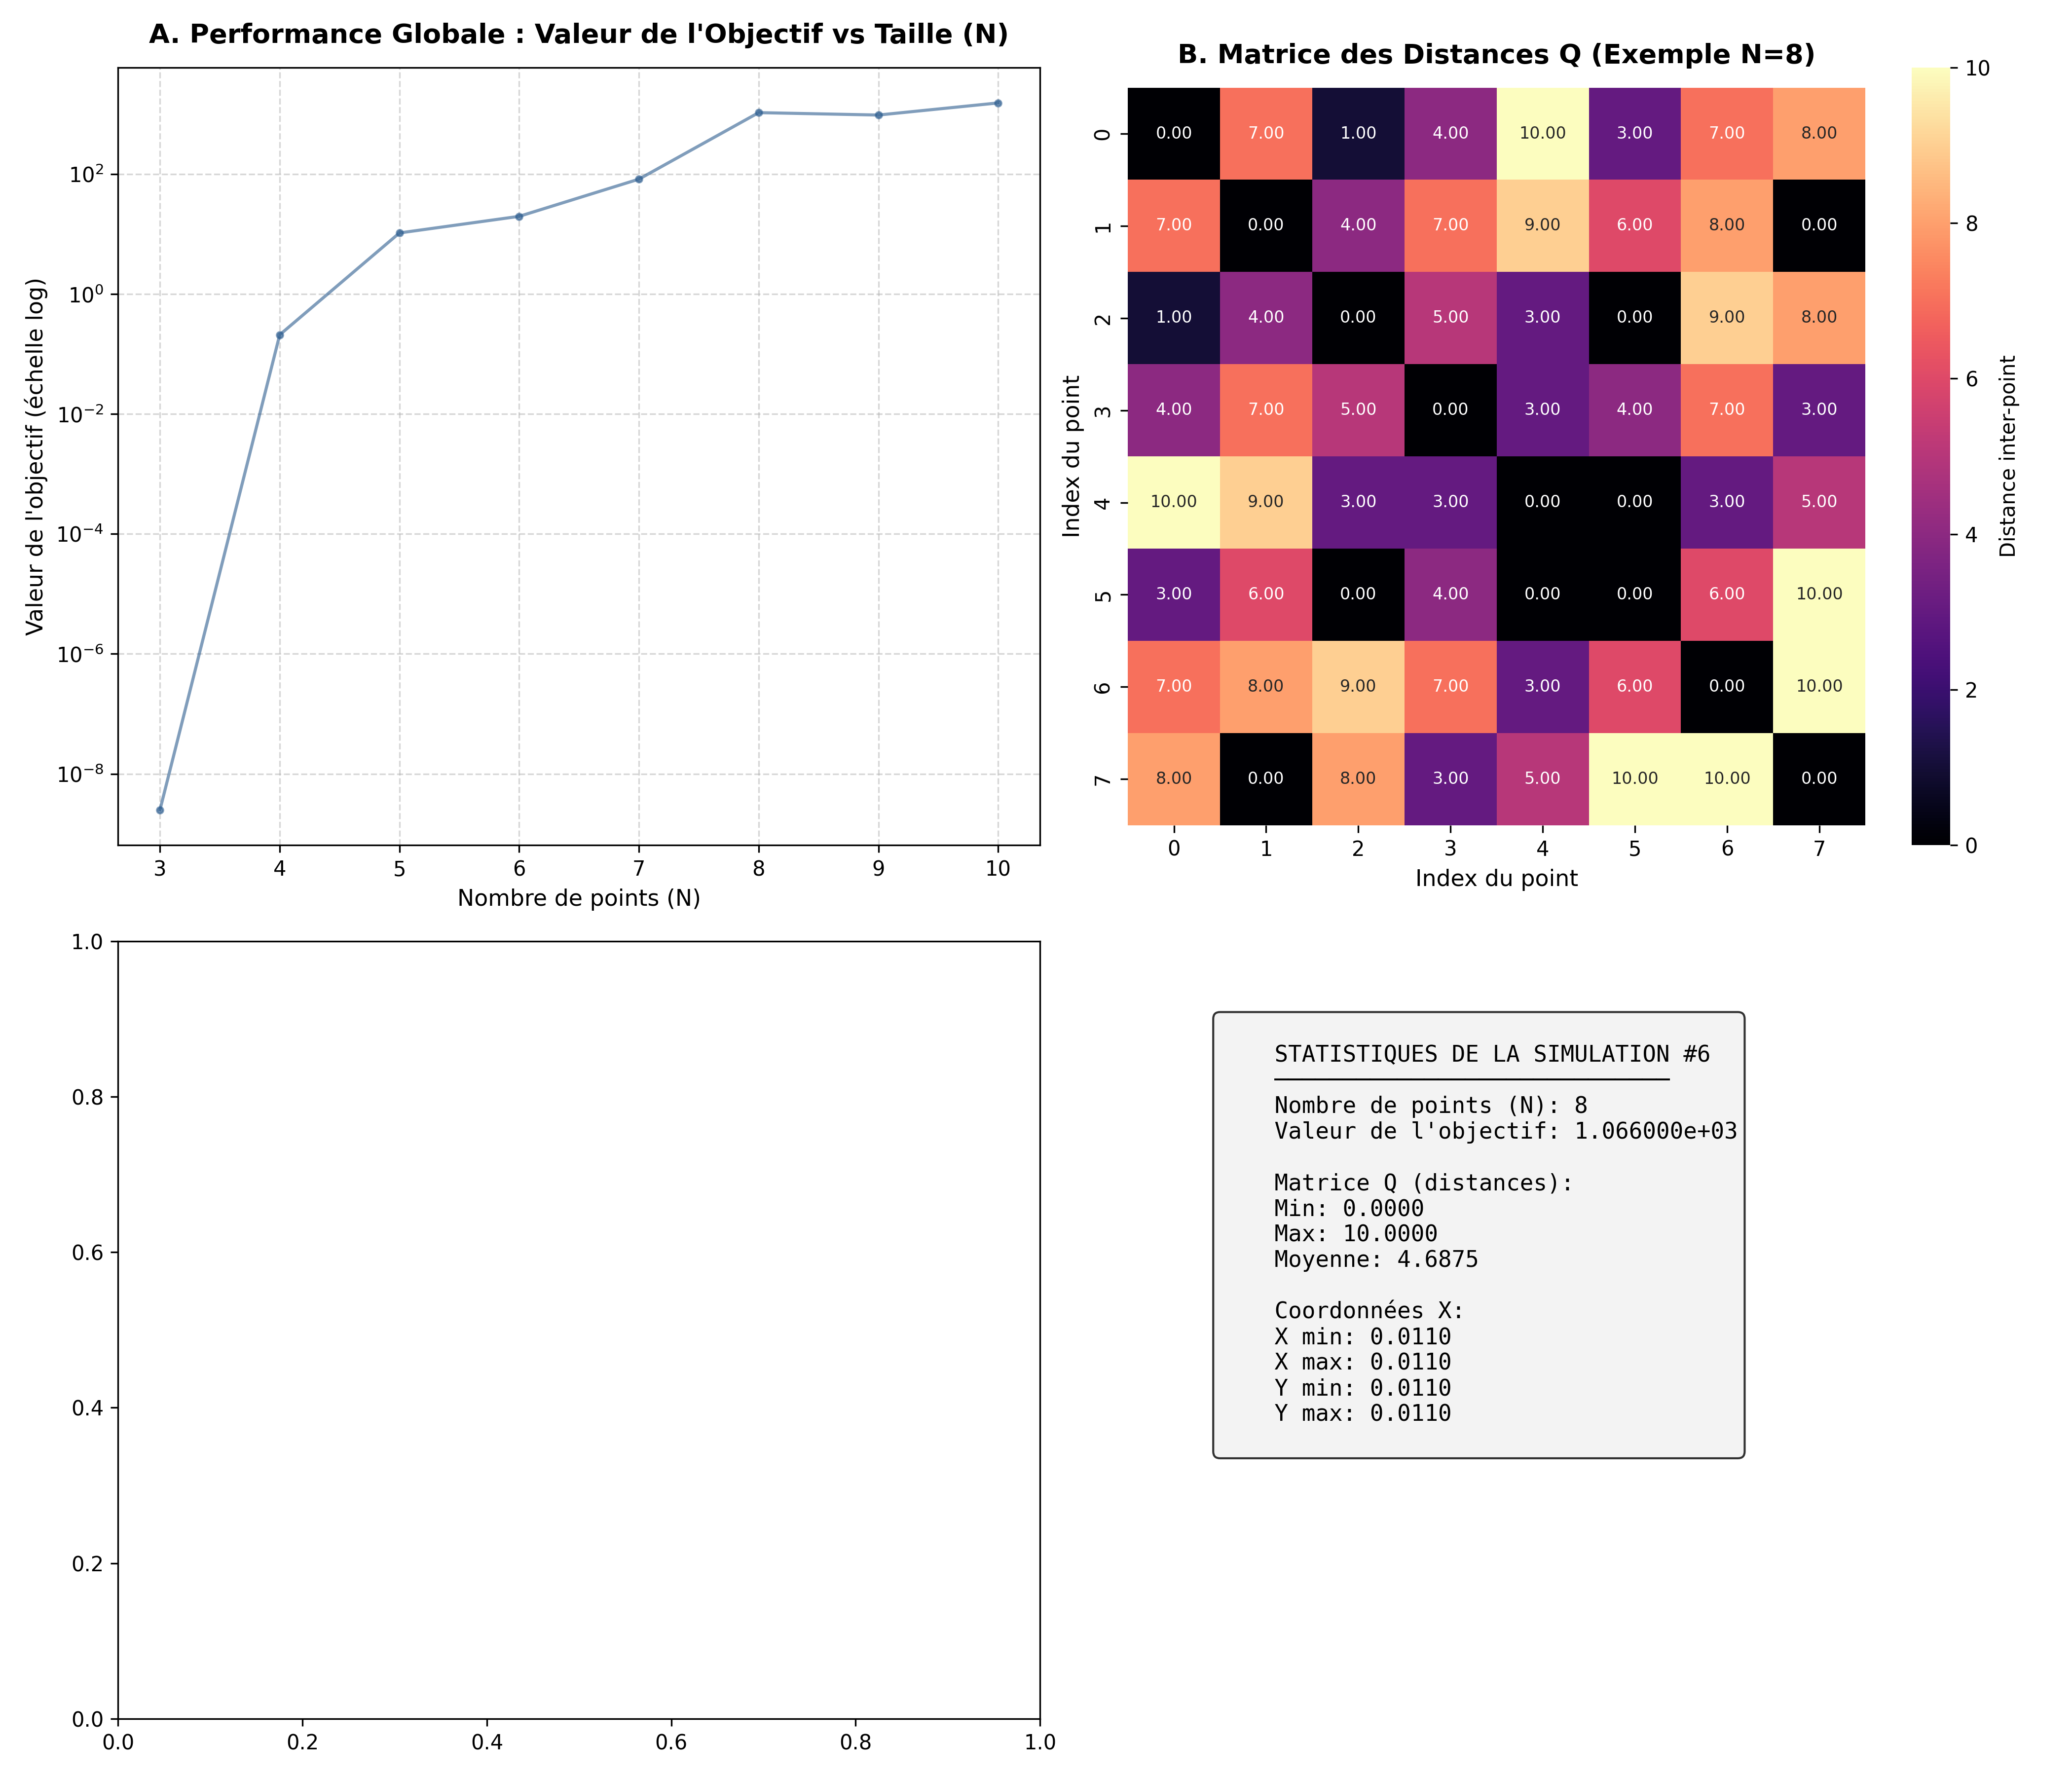
\includegraphics[width=\textwidth]{dashboard_results_optimization_form2.png}
  \caption{Tableau de bord pour la Formulation 2 (variables auxiliaires
    $y_{ij}$, $z_{ij}$).  Comparaison des performances entre V1 ($Q$
    aleatoire) et V2 (verite terrain avec warm-start).}
\end{figure}

\subsection{Top 10 des meilleures simulations}

\begin{figure}[H]
  \centering
  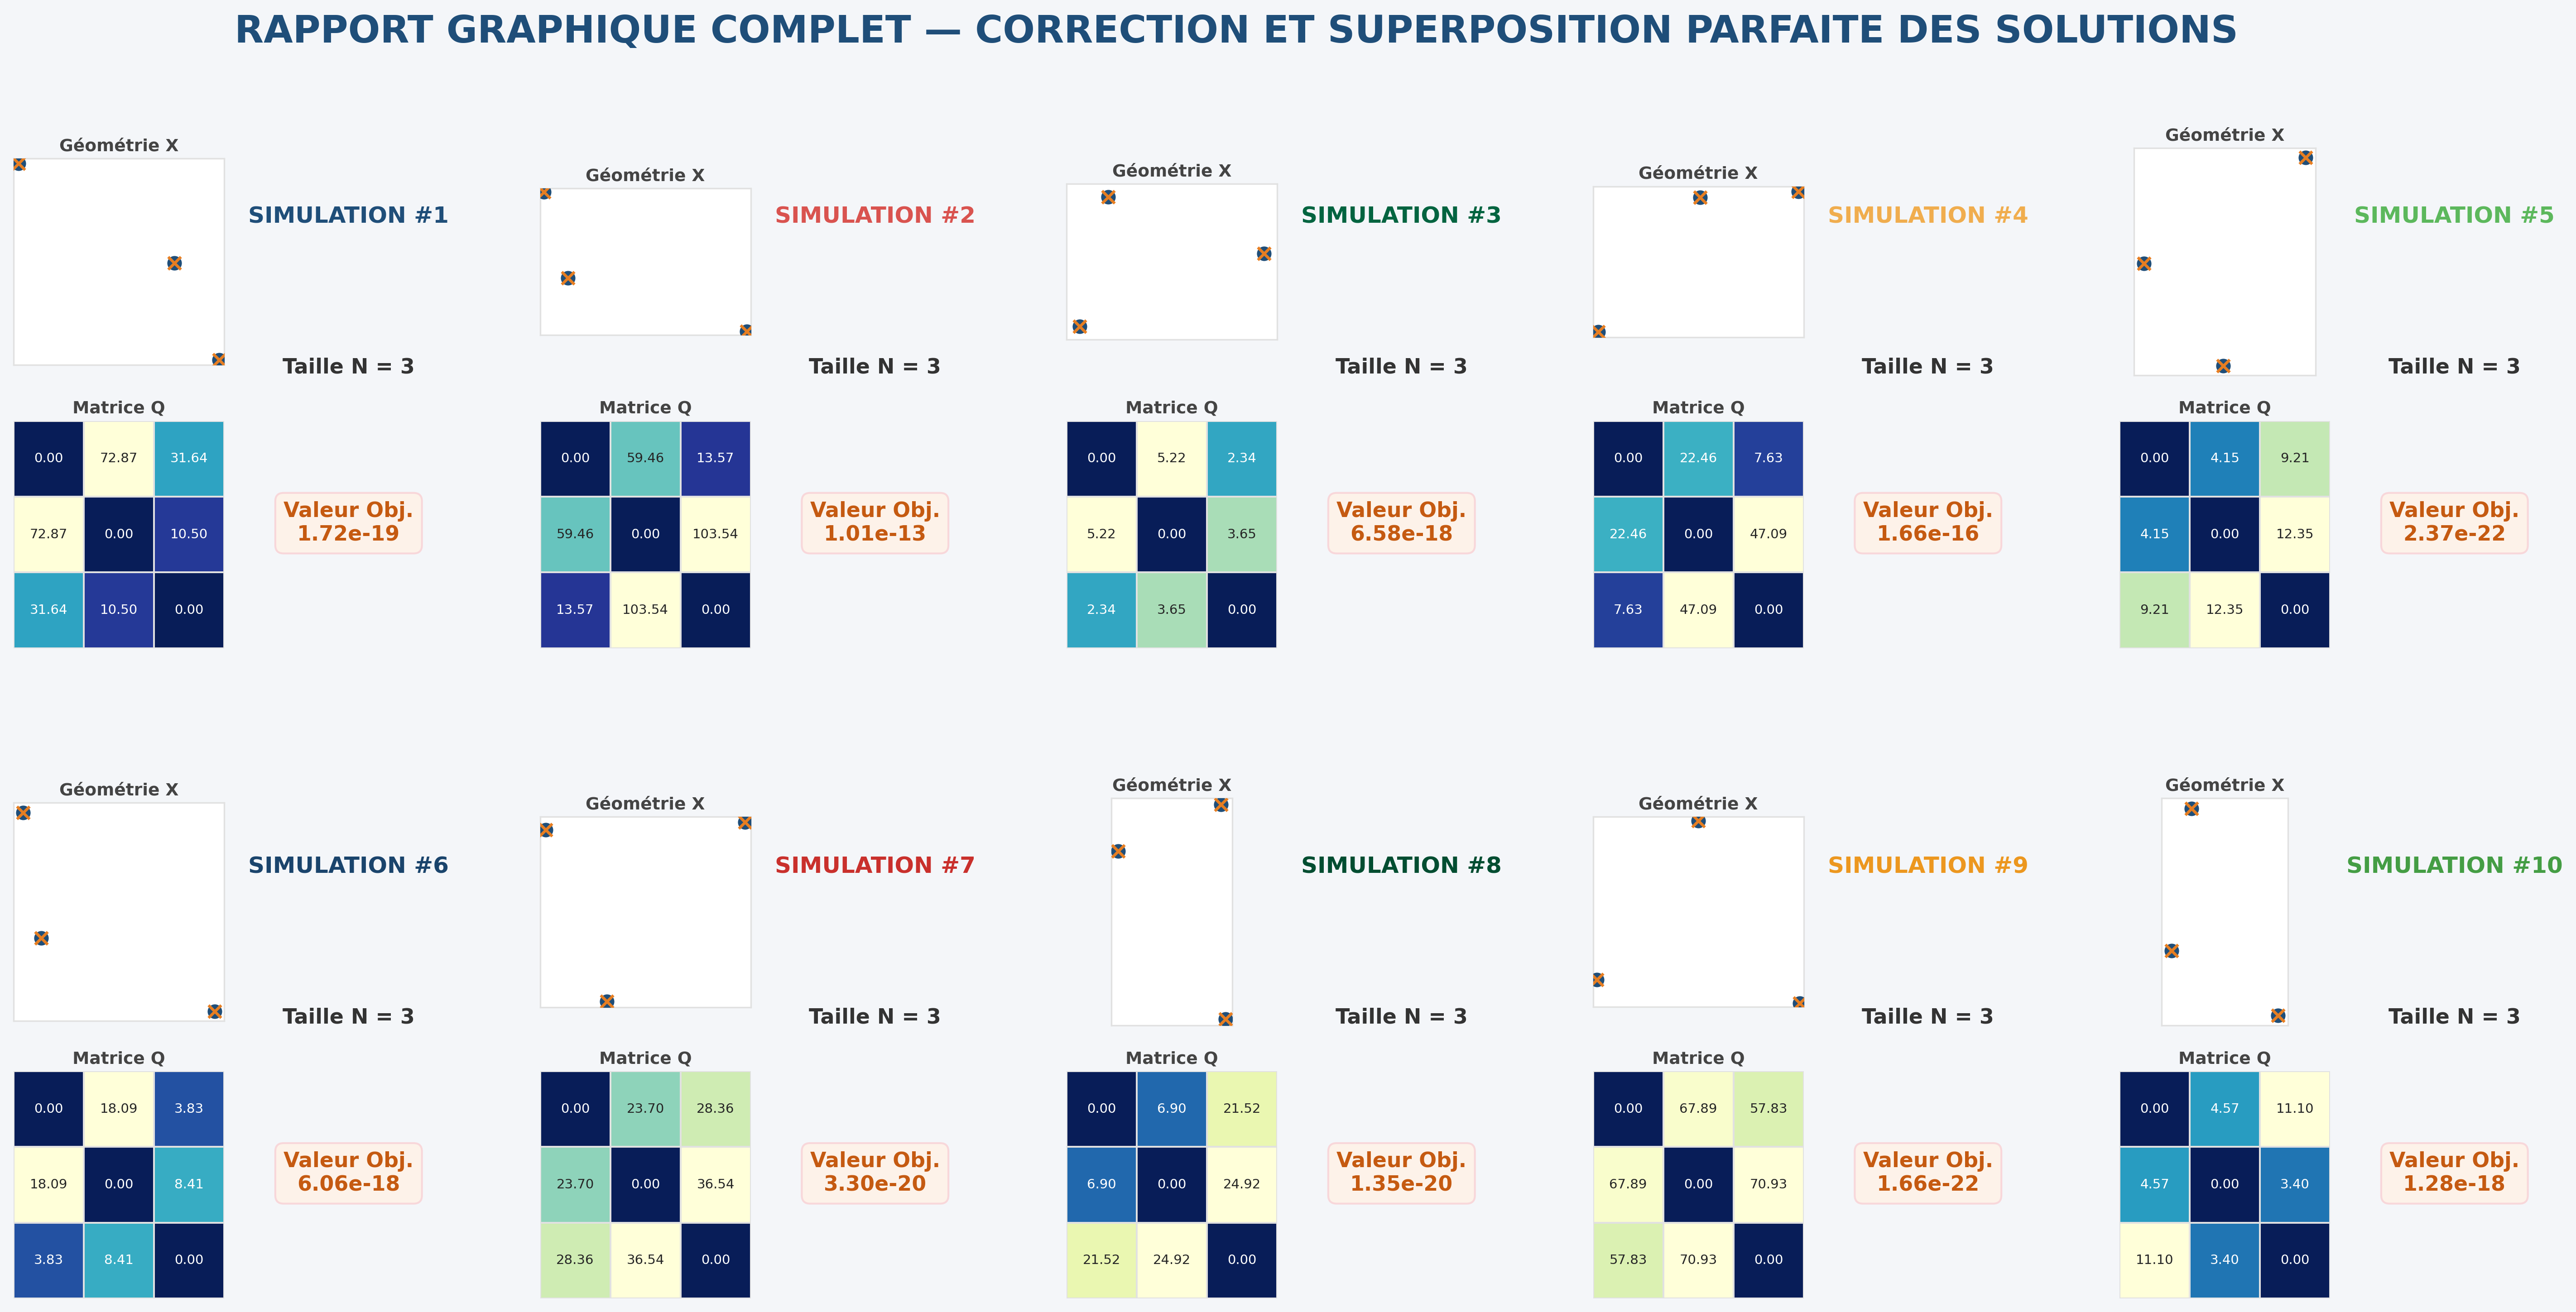
\includegraphics[width=\textwidth]{dashboard_top10_simulations.png}
  \caption{Top 10 des simulations avec les valeurs d'objectif les plus
    faibles.  Ces configurations correspondent aux instances pour
    lesquelles Ipopt a converge le plus precisement.}
\end{figure}

\subsection{Tableau brut des simulations}

\begin{figure}[H]
  \centering
  
\includegraphics[width=\textwidth]{tableau_simulations_pur.png}
  \caption{Tableau complet de toutes les simulations executees : chaque
    ligne correspond a une instance ($n$, tirage), avec la valeur de
    l'objectif atteinte et le statut de terminaison du solveur.}
\end{figure}

\newpage

%% ════════════════════════════════════════════════════════════════════════
\section{Analyse comparative}
%% ════════════════════════════════════════════════════════════════════════

\subsection{Recapitulatif des formulations}

\begin{table}[H]
\centering
\begin{tabularx}{\linewidth}{lXXX}
\toprule
\textbf{Version} & \textbf{Objectif} & \textbf{Matrice $Q$}
  & \textbf{Convergence} \\
\midrule
F1-G1 &
  $\sum_{i<j}(\|\Delta\mathbf{x}_{ij}\|^2 - Q_{ij}^2)^2$ &
  Aleatoire continu &
  Bonne (sans reference) \\
F1-G2 &
  $\sum_{i<j}(\|\Delta\mathbf{x}_{ij}\|^2 - Q_{ij})^2$ &
  Distances au carre reelles &
  Excellente ($\sim 10^{-19}$) \\
F2-V1 &
  $\sum_{i<j}(y_{ij}+z_{ij}-Q_{ij}^2)^2$ &
  Entiers discrets &
  Variable \\
F2-V2 &
  $\sum_{i<j}(y_{ij}+z_{ij}-Q_{ij}^2)^2$ &
  Distance euclidienne &
  Bonne \\
\bottomrule
\end{tabularx}
\caption{Synthese des quatre formulations testees.}
\end{table}

\subsection{Points cles}

\begin{enumerate}
  \item \textbf{Invariances geometriques.}
    Le probleme de distances est invariant par isometrie
    (translation, rotation, reflexion symetrique).
    Sans contraintes d'ancrage, le solveur peut converger vers une
    solution translatee ou reflechie, mathematiquement equivalente mais
    physiquement differente.

  \item \textbf{Non-convexite.}
    Les quatre formulations conduisent a un probleme non convexe
    (objectif quartique en $\mathbf{x}$).
    Ipopt garantit uniquement la convergence vers un
    \textbf{minimum local}.
    La qualite de la solution depend fortement de l'initialisation.

  \item \textbf{Coherence de $Q$.}
    Seules F1-G2 et F2-V2 utilisent une matrice $Q$ coherente
    (construite a partir de vraies positions).
    Les formulations avec $Q$ aleatoire peuvent produire des systemes
    \textit{irrealisables} pour lesquels l'objectif ne peut pas
    atteindre zero.

  \item \textbf{Variables auxiliaires.}
    L'introduction de $y_{ij}$, $z_{ij}$ dans F2 ameliore le
    conditionnement numerique mais augmente le nombre de variables et
    de contraintes : $2\binom{n}{2}$ variables et contraintes
    supplementaires pour $n$ atomes en 2D.
\end{enumerate}

%% ════════════════════════════════════════════════════════════════════════
\section{Conclusion et perspectives}
%% ════════════════════════════════════════════════════════════════════════

\subsection{Bilan}

Ce travail a permis de construire et tester quatre formulations du
probleme de positionnement d'atomes en Julia avec JuMP/Ipopt.
Les resultats montrent que :

\begin{itemize}
  \item La formulation \textbf{F1-G2} offre les meilleures performances
    numeriques (objectif $\sim 10^{-19}$) lorsque $Q$ est coherent avec
    une verite terrain.
  \item L'introduction des variables auxiliaires (\textbf{F2}) offre une
    meilleure structure pour des extensions futures (relaxations,
    decomposition), au prix d'un probleme legerement plus grand.
  \item La graine aleatoire fixe (\texttt{Random.seed!(2024)}) assure la
    reproductibilite des experiences.
\end{itemize}

\subsection{Perspectives}

\begin{itemize}
  \item \textbf{Relaxation SDP :} reformuler le probleme de distances
    comme un programme semi-defini positif pour obtenir des bornes
    globales certifiees.
  \item \textbf{Extension 3D :} en dimension $d=3$, des ancres
    supplementaires (6 degres de liberte a fixer) sont necessaires pour
    lever toutes les ambiguites geometriques.
  \item \textbf{Robustesse au bruit :} tester les formulations avec
    $Q_{ij} + \varepsilon$ ($\varepsilon \sim \mathcal{N}(0,\sigma^2)$)
    pour simuler des mesures experimentales imparfaites.
  \item \textbf{Initialisation MDS :} utiliser le
    \textit{Multidimensional Scaling} spectral classique comme
    warm-start de qualite, sans necessiter la verite terrain.
\end{itemize}

\end{document}
